\documentclass[a4paper,10pt]{article}
\usepackage[utf8x]{inputenc}
\usepackage{amsmath}
\usepackage{graphicx}
\usepackage[english]{babel}
\usepackage{url}
\usepackage{epstopdf}
\usepackage{subfig}
\usepackage{graphicx}

\title{Procesamiento Avanzado de Imágenes\\IEE3784}
\author{\textbf{Tarea 01}\\Norman F. Sáez\\nfsaez@uc.cl}
\date{\today}

\begin{document}
\maketitle
\section{Pregunta 1}
Se utiliza el algoritmo de Cox de Boor para calcular tanto las bases como
b-splines, de acuerdo a los puntos de control entregados en la tarea y el
vector de nodos.  Se considera que en cada iteración, se hacen 5 sumas y  2
multiplicaciones por coordenada ``x'', de esta manera, para 100 puntos un resultado de
144 sumas por coordenada ``x'' y 60 multiplicaciones por
coordenada ``x''. El total por coordenada es de \textbf{\textit{288
sumas}} y \textbf{\textit{120 multiplicaciones}}, por cada \textbf{100 puntos}.
El total de la curva de 400 puntos es de 1152 sumas y de 480 multiplicaciones.

\begin{figure}[ht!]
  \centering
  \subfloat[B-Splines: Puntos de control en azul]{\label{fig:img1a}\includegraphics[width=0.50\textwidth]{img/img1a.eps}}
  ~ 
  \subfloat[Bases $B_{4,1}=rojo$, $B_{4,2}=verde$, $B_{4,3}=azul$, $B_{4,4}=magenta$]{\label{fig:img1b}\includegraphics[width=0.50\textwidth]{img/img1b.eps}}
  ~ 
  \caption{B-Splines y Bases}
  \label{fig:p1}
\end{figure}

\section{Pregunta 2}
\begin{figure}[ht!]
  \centering
  \subfloat[B-Spline Forma Polar: Puntos de control en azul]{\label{fig:img2}\includegraphics[width=0.80\textwidth]{img/img2.eps}}
  ~ 
  \caption{B-Splines calculado en forma polar}
  \label{fig:p2}
\end{figure}

\section{Pregunta 3}
%\begin{figure}[ht!]
%  \centering
%  \subfloat[]{\label{fig:img3}\includegraphics[width=0.80\textwidth]{img/img3.eps}}
%  ~ 
%  \caption{}
%  \label{fig:p3}
%\end{figure}

\section{Pregunta 4}
\begin{figure}[ht!]
  \centering
  \subfloat[B-Spline, Casteljau: Puntos de control en azul]{\label{fig:img4}\includegraphics[width=0.80\textwidth]{img/img4.eps}}
  ~ 
  \caption{B-Splines calculado usando Casteljau}
  \label{fig:p4}
\end{figure}

\end{document}
